\documentclass[12pt]{article}

\usepackage{amsmath}
\usepackage{amssymb}
\usepackage[dvips]{graphicx}
\usepackage{eepic}
\usepackage{color}
\usepackage{wasysym} % \female \male
\usepackage[landscape,pdftex]{geometry}
\usepackage{fancyhdr}
\usepackage{wasysym} % for check symbol
\usepackage{hyperref}

\DeclareOption{bigsym}{\DeclareSymbolFont{largesymbols}{OMX}{psycm}{m}{n}}
\ProcessOptions

\setlength{\oddsidemargin}{-0.75in}
\setlength{\evensidemargin}{-0.75in}
\setlength{\topmargin}{-1in}
\setlength{\textheight}{7.75in}
\setlength{\textwidth}{10.5in}
\setlength{\footskip}{0in}
\setlength{\parindent}{0pt}
\setlength{\rightskip}{0pt plus 1fil} % makes ragged right

\renewcommand{\familydefault}{phv} % helvetica

% following: color
\definecolor{bgcolor}{rgb}{0.1,0.1,0.1}
\definecolor{yellow}{rgb}{1,1,0.4}
\definecolor{blue}{rgb}{0.4,0.8,1}
\definecolor{pink}{rgb}{1,0.4,1}
\definecolor{hotpink}{rgb}{1,0,0.5}
\definecolor{white}{rgb}{1,1,1}
\definecolor{gray}{rgb}{0.6,0.6,0.6}
\hypersetup{pdfpagemode=UseNone} % don't show bookmarks on initial view
\hypersetup{colorlinks, urlcolor={blue}}

% header/footer layout
\pagestyle{fancy}
\lhead{} \chead{} \rhead{}
\lfoot{} \cfoot{} \rfoot{\color{gray} \thepage}
\renewcommand{\headrulewidth}{0pt}
\renewcommand{\footrulewidth}{0pt}

% font sizes
\newcommand{\superlarge}{\fontsize{60}{60} \selectfont}
\newcommand{\titlesize}{\fontsize{40}{50} \selectfont}
\newcommand{\headsize}{\fontsize{35}{35} \selectfont}
\newcommand{\textsize}{\fontsize{30}{35} \selectfont}
\newcommand{\smallsize}{\fontsize{25}{30} \selectfont}
\newcommand{\smallersize}{\fontsize{20}{25} \selectfont}
\newcommand{\smallestsize}{\fontsize{18}{22} \selectfont}
\newcommand{\evensmaller}{\fontsize{14}{18} \selectfont}
\newcommand{\lod}{\text{LOD}}
\newcommand{\bic}{\text{BIC}}
\newcommand{\rss}{\text{RSS}}
\newcommand{\var}{\text{var}}
\newcommand{\M}{\text{M}}
%\renewcommand{\log}{\text{log}}
%\renewcommand{\max}{\text{max}}



\pagecolor{bgcolor}
\color{white}

\begin{document}

\thispagestyle{empty}

\begin{center}
\titlesize \color{yellow}

\vspace*{24.5mm}

{\headsize Creating effective figures and tables}

\vspace*{14.5mm}

\color{pink}
\rule{10in}{1mm}
%\vspace{-10mm}

\vspace{10mm}

\textsize \color{blue}
Karl W Broman
\vspace{5mm}

{\smallersize Biostatistics \& Medical Informatics

University of Wisconsin -- Madison
\vspace{20mm}


\href{http://www.biostat.wisc.edu/~kbroman}{\tt biostat.wisc.edu/{\textasciitilde}kbroman} \\
\href{http://github.com/kbroman}{\tt github.com/kbroman} \\
\href{https://twitter.com/kwbroman}{\tt @kwbroman}

}

\end{center}


\newpage

\headsize \color{yellow}
\hfill \begin{minipage}{5.75in}
\centering
The top ten worst graphs
\end{minipage}

\vspace{30mm}
\smallsize \color{white}

\hspace{0.5in} \begin{minipage}{9in}

\setlength{\rightskip}{0pt plus 1fil} % makes ragged right

With apologizes to the authors, we provide the following list of the
top ten worst graphs in the scientific literature.

\vspace{15mm}

As these examples indicate, good scientists can make mistakes.

\vspace{35mm}

\hfill \color{blue} \smallersize
\href{http://bit.ly/TopTenWorstGraphs}{\tt bit.ly/TopTenWorstGraphs}

\end{minipage}

\newpage
\thispagestyle{empty}

\headsize \color{yellow}
\hfill \begin{minipage}{5.75in}
\centering
10
\end{minipage}

\vspace{30mm}

\centerline{\includegraphics[height=5in]{TopTenWorstGraphs/broman_fig1.jpg}}

\vfill \hfill \smallestsize \color{blue}
Broman et al., Am J Hum Genet 63:861-869, 1998, Fig. 1

\newpage
\thispagestyle{empty}


\headsize \color{yellow}
\hfill \begin{minipage}{5.75in}
\centering
9
\end{minipage}

\vspace{30mm}

\centerline{\includegraphics[height=5in]{TopTenWorstGraphs/cotter_fig2.jpg}}

\vfill \hfill \smallestsize \color{blue}
Cotter et al., J Clin Epidemiol 57:1086-1095, 2004, Fig 2

\newpage
\thispagestyle{empty}


\headsize \color{yellow}
\hfill \begin{minipage}{5.75in}
\centering
8
\end{minipage}

\vspace{30mm}

\centerline{\includegraphics[height=5in]{TopTenWorstGraphs/jorgenson_fig2a.jpg}}

\vfill \hfill \smallestsize \color{blue}
Jorgenson et al., Am J Hum Genet 76:276-290, 2005, Fig 2

\newpage
\thispagestyle{empty}

\headsize \color{yellow}
\hfill \begin{minipage}{5.75in}
\centering
7
\end{minipage}

\vspace{30mm}

\centerline{\includegraphics[height=5in]{TopTenWorstGraphs/kim_fig1.png}}

\vfill \hfill \smallestsize \color{blue}
Kim et al., Nutr Res Prac 6:120-125, 2012
Fig 1

\newpage
\thispagestyle{empty}


\headsize \color{yellow}
\hfill \begin{minipage}{5.75in}
\centering
6
\end{minipage}

\vspace{30mm}

\centerline{\includegraphics[height=5in]{TopTenWorstGraphs/cawley_fig1.jpg}}

\vfill \hfill \smallestsize \color{blue}
Cawley et al., Cell 116:499-509, 2004, Fig 1

\newpage
\thispagestyle{empty}


\headsize \color{yellow}
\hfill \begin{minipage}{5.75in}
\centering
5
\end{minipage}

\vspace{30mm}

\centerline{\includegraphics[height=5in]{TopTenWorstGraphs/hummer_fig4.jpg}}

\vfill \hfill \smallestsize \color{blue}
Hummer et al., J Virol 75:7774-7777, 2001, Fig 4

\newpage
\thispagestyle{empty}


\headsize \color{yellow}
\hfill \begin{minipage}{5.75in}
\centering
4
\end{minipage}

\vspace{30mm}

\centerline{\includegraphics[height=5in]{TopTenWorstGraphs/epstein_fig1.jpg}}


\vfill \hfill \smallestsize \color{blue}
Epstein and Satten, Am J Hum Genet 73:1316-1329, 2003, Fig 1

\newpage
\thispagestyle{empty}


\headsize \color{yellow}
\hfill \begin{minipage}{5.75in}
\centering
3
\end{minipage}

\vspace{30mm}


\centerline{\includegraphics[height=5in]{TopTenWorstGraphs/mykland_fig1.jpg}}
\vfill \hfill \smallestsize \color{blue}
Mykland et al., J Am Stat Asso 90:233-241, 1995, Fig 1

\newpage
\thispagestyle{empty}


\headsize \color{yellow}
\hfill \begin{minipage}{5.75in}
\centering
2
\end{minipage}

\vspace{30mm}

\centerline{\includegraphics[height=5in]{TopTenWorstGraphs/wittke_thompson_fig1CD.jpg}}

\vfill \hfill \smallestsize \color{blue}
Wittke-Thompson et al., Am J Hum Genet 76:967-986, Fig 1

\newpage
\thispagestyle{empty}


\headsize \color{yellow}
\hfill \begin{minipage}{5.75in}
\centering
1
\end{minipage}

\vspace{30mm}

\centerline{\includegraphics[height=5in]{TopTenWorstGraphs/roeder_fig4.jpg}}


\vfill \hfill \smallestsize \color{blue}
Roeder, Stat Sci 9:222-278, 1994, Fig 4


\newpage


\headsize \color{yellow}
\hfill \begin{minipage}{5.75in}
\centering
Displaying data well
\end{minipage}

\vspace{30mm}
\smallsize \color{white}

\hspace{0.5in} \begin{minipage}[t]{9in}
\begin{itemize}

\itemsep24pt

\item Be accurate and clear.

\item Let the data speak.

{\color{blue} \smallersize
\begin{itemize}
\item Show as much information as possible, taking care not to
  obscure the message.
\end{itemize} }

\item Science not sales.

{\color{blue} \smallersize
\begin{itemize}
\item Avoid unnecessary frills (esp. gratuitous 3d).
\end{itemize} }

\item In tables, every digit should be meaningful. Don't drop ending 0's.

\end{itemize}
\end{minipage}


\newpage

\headsize \color{yellow}
\hfill \begin{minipage}{5.75in}
\centering
Things not to do
\end{minipage}

\vspace{35mm}
\smallsize \color{white}


\hfill \begin{minipage}{9.6in}
\color{white}
\begin{itemize}
\item Display as little information as possible.
\item Obscure what you do show (with chart junk).
\item Use pseudo-3d and color gratuitously.
\item Make a pie chart (preferably in color and 3d).
\item Use a poorly chosen scale.
\item Ignore sig figs.
\end{itemize}
\end{minipage}



\newpage


\headsize \color{yellow}
\hfill \begin{minipage}{5.75in}
\centering
Show the data
\end{minipage}

\vspace{30mm}

\begin{minipage}[t]{4.5in}
\vspace*{0cm}

\includegraphics[width=4.5in]{Figs/fig1a.png}
\end{minipage}
\hfill
\begin{minipage}[t]{4.5in}
\vspace*{0cm}

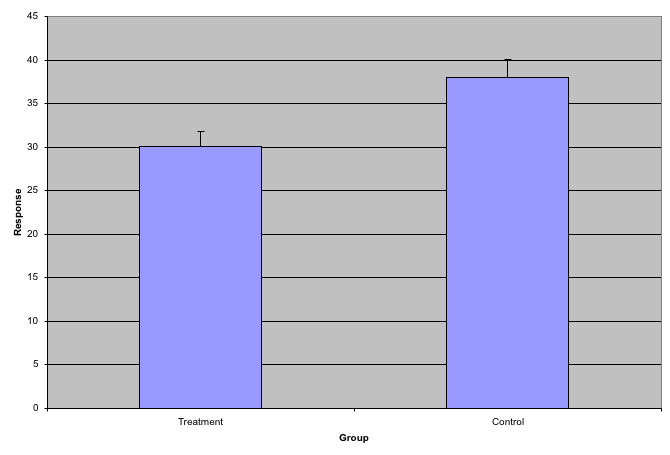
\includegraphics[width=4.5in]{Figs/fig1c.png}
\end{minipage}



\newpage

\addtocounter{page}{-1}

\headsize \color{yellow}
\hfill \begin{minipage}{5.75in}
\centering
Show the data
\end{minipage}

\vspace{30mm}

\begin{minipage}[t]{4.5in}
\vspace*{0cm}

\includegraphics[width=4.5in]{Figs/fig1a.png}
\end{minipage}
\hfill
\begin{minipage}[t]{4.5in}
\vspace*{0cm}

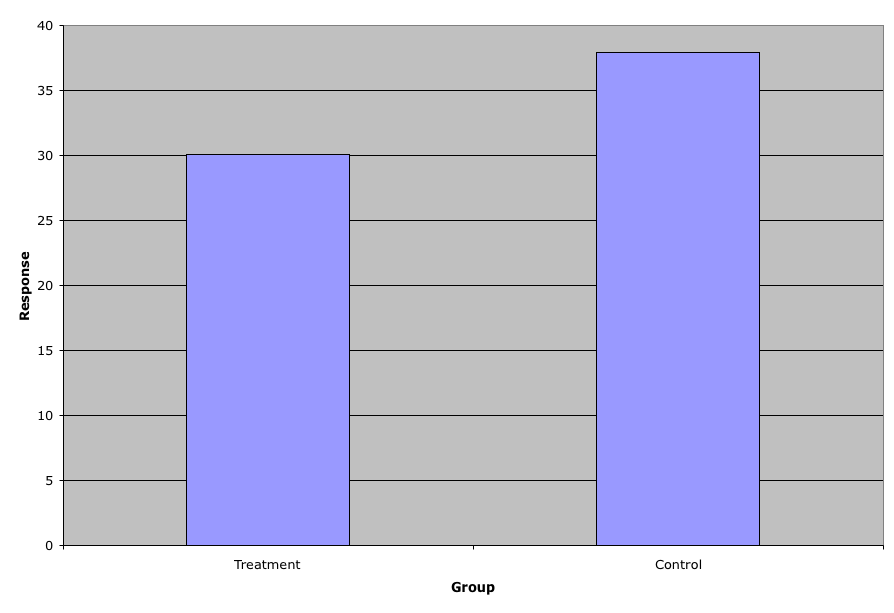
\includegraphics[width=4.5in]{Figs/fig1d.png}
\end{minipage}



\newpage

\addtocounter{page}{-1}

\headsize \color{yellow}
\hfill \begin{minipage}{5.75in}
\centering
Show the data
\end{minipage}

\vspace{30mm}

\begin{minipage}[t]{4.5in}
\vspace*{0cm}

\includegraphics[width=4.5in]{Figs/fig1a.png}
\end{minipage}
\hfill
\begin{minipage}[t]{4.5in}
\vspace*{0cm}

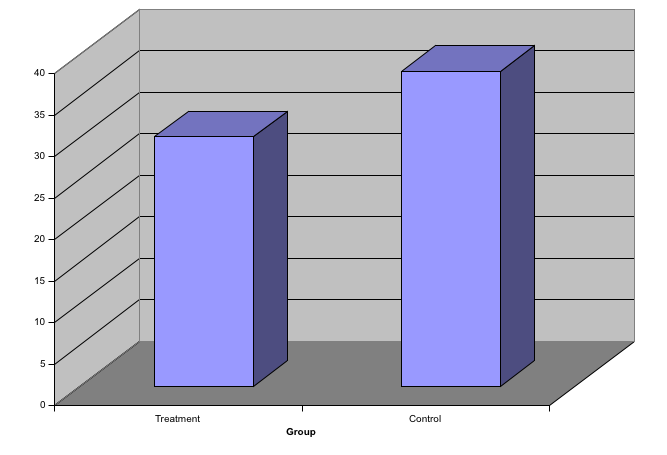
\includegraphics[width=4.5in]{Figs/fig1e.png}
\end{minipage}



\newpage


\headsize \color{yellow}
\hfill \begin{minipage}{5.75in}
\centering
Consider logs
\end{minipage}

\vspace{30mm}

\begin{minipage}[t]{4.5in}
\vspace*{0cm}

\includegraphics[width=4.5in]{Figs/fig3a.png}
\end{minipage}
\hfill
\begin{minipage}[t]{4.5in}
\vspace*{0cm}

\includegraphics[width=4.5in]{Figs/fig3b.png}
\end{minipage}


\newpage

\addtocounter{page}{-1}

\headsize \color{yellow}
\hfill \begin{minipage}{5.75in}
\centering
Consider logs
\end{minipage}

\vspace{30mm}

\begin{minipage}[t]{4.5in}
\vspace*{0cm}

\includegraphics[width=4.5in]{Figs/fig3a.png}
\end{minipage}
\hfill
\begin{minipage}[t]{4.5in}
\vspace*{0cm}

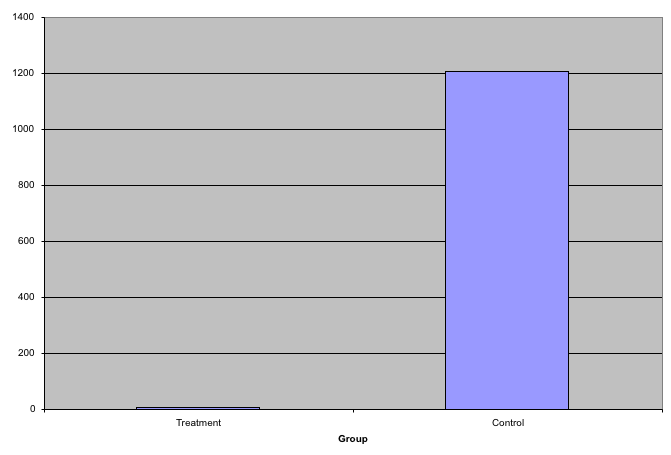
\includegraphics[width=4.5in]{Figs/fig3c.png}
\end{minipage}


\newpage

\addtocounter{page}{-1}

\headsize \color{yellow}
\hfill \begin{minipage}{5.75in}
\centering
Consider logs
\end{minipage}

\vspace{30mm}

\begin{minipage}[t]{4.5in}
\vspace*{0cm}

\includegraphics[width=4.5in]{Figs/fig3a.png}
\end{minipage}
\hfill
\begin{minipage}[t]{4.5in}
\vspace*{0cm}

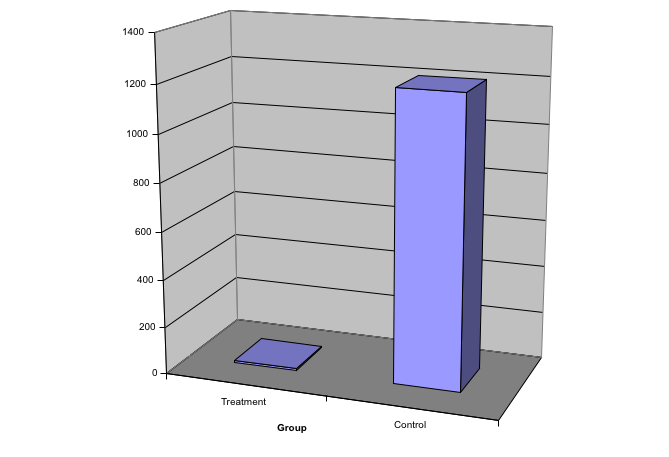
\includegraphics[width=4.5in]{Figs/fig3d.png}
\end{minipage}




\newpage


\headsize \color{yellow}
\hfill \begin{minipage}{5.75in}
\centering
Consider logs
\end{minipage}

\vspace{30mm}

\centerline{\includegraphics[height=6in]{Figs/fig5c.png}}


\newpage

\addtocounter{page}{-1}

\headsize \color{yellow}
\hfill \begin{minipage}{5.75in}
\centering
Consider logs
\end{minipage}

\vspace{30mm}

\centerline{\includegraphics[height=6in]{Figs/fig5d.png}}

\newpage

\addtocounter{page}{-1}

\headsize \color{yellow}
\hfill \begin{minipage}{5.75in}
\centering
Consider logs
\end{minipage}

\vspace{30mm}

\centerline{\includegraphics[height=6in]{Figs/fig5e.png}}

\newpage

\addtocounter{page}{-1}

\headsize \color{yellow}
\hfill \begin{minipage}{5.75in}
\centering
Consider logs
\end{minipage}

\vspace{30mm}

\centerline{\includegraphics[height=6in]{Figs/fig5f.png}}

\newpage

\addtocounter{page}{-1}

\headsize \color{yellow}
\hfill \begin{minipage}{5.75in}
\centering
Consider logs
\end{minipage}

\vspace{30mm}

\centerline{\includegraphics[height=6in]{Figs/fig5d.png}}

\newpage

\addtocounter{page}{-1}

\headsize \color{yellow}
\hfill \begin{minipage}{5.75in}
\centering
Consider logs
\end{minipage}

\vspace{30mm}

\centerline{\includegraphics[height=6in]{Figs/fig5b.png}}

\newpage


\headsize \color{yellow}
\hfill \begin{minipage}{5.75in}
\centering
Take differences
\end{minipage}

\vspace{30mm}

\centerline{\includegraphics[height=6in]{Figs/fig5a.png}}




\newpage

\headsize \color{yellow}
\hfill \begin{minipage}{5.75in}
\centering
A bad table
\end{minipage}

\vspace{30mm}

\centerline{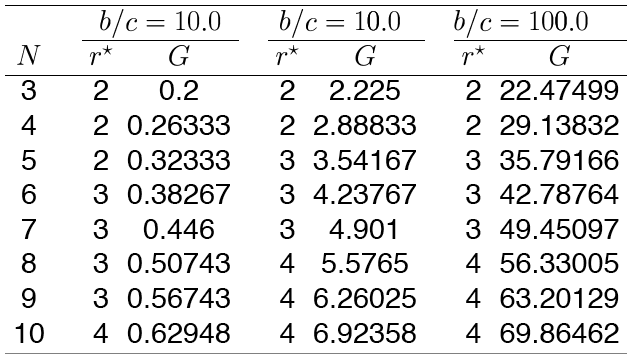
\includegraphics[width=8in]{Figs/tableB.png}}


\newpage


\headsize \color{yellow}
\hfill \begin{minipage}{5.75in}
\centering
An improved table
\end{minipage}

\vspace{30mm}

\centerline{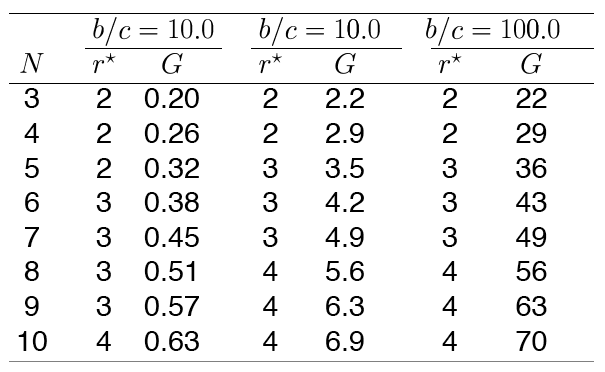
\includegraphics[width=8in]{Figs/tableA.png}}

\newpage


\headsize \color{yellow}
\hfill \begin{minipage}{5.75in}
\centering
Further reading
\end{minipage}

\vspace{30mm}
\smallestsize \color{white}

\hspace{0.5in} \begin{minipage}[t]{9in}
\begin{itemize}

\itemsep12pt

\item ER Tufte (1983) The visual display of quantitative information.
Graphics Press.
\item ER Tufte (1990) Envisioning information. Graphics Press.
\item ER Tufte (1997) Visual explanations. Graphics Press.

\vspace*{8mm}

\item A Gelman, C Pasarica, R Dodhia (2002) Let's practice what we preach:
Turning tables into graphs. The American Statistician 56:121-130

\vspace*{8mm}

\item Robbins NB (2004) Creating more effective graphs. Wiley

\vspace*{8mm}

\item Nature Methods columns: \href{http://bang.clearscience.info/?p=546}{\tt http://bang.clearscience.info/?p=546}

\end{itemize}
\end{minipage}


\end{document}
